% -*- coding: utf-8 -*-
\documentclass{beamer}
\usepackage[utf8]{inputenc}

\usetheme{complang}

% Have Page n/N in the lower left corner
% \setbeamertemplate{footline}
% {%
% \begin{beamercolorbox}[wd=0.5\textwidth,ht=3ex,dp=1.5ex,
%    leftskip=.5em,rightskip=.5em]{author in head/foot}%
% \usebeamerfont{author in head/foot}%
% \insertframenumber/\inserttotalframenumber\hfill\insertshortauthor%
% \end{beamercolorbox}%
% \vspace*{-4.5ex}\hspace*{0.5\textwidth}%
% \begin{beamercolorbox}[wd=0.5\textwidth,ht=3ex,dp=1.5ex,
%    left,leftskip=.5em]{title in head/foot}%
% \usebeamerfont{title in head/foot}%
% \insertshorttitle%
% \end{beamercolorbox}%
% }

%\usepackage{pifont}
%\usepackage{amstext}
\usepackage{amsmath}
%\usepackage{logic}
% \usepackage{proof}
\usepackage{xcolor}
\usepackage{listings}
\usepackage{hyperref}
\usepackage{booktabs}
\usepackage{tikz}
\usetikzlibrary{arrows,automata,positioning}
\usetikzlibrary{fit}
\usepackage{drawproof}

% Colors
\definecolor{myblue}{rgb}{0.089, 0.089, 0.58}
\definecolor{myred}{rgb}{0.77, 0.05, 0.16}
\definecolor{mygreen}{rgb}{0.05, 0.77, 0.16}
\definecolor{myyellow}{rgb}{0.77, 0.77, 0.16}
\definecolor{vertfonce}{HTML}{347003}

\setbeamercolor{local structure}{fg=black}

% Arrows
\newcommand{\redarrow}{{\color{myred} \Pisymbol{pzd}{217}}}
\newcommand{\redresarrow}{{\large\color{myred} \Pisymbol{pzd}{229}}}
\newcommand{\ra}{\hspace{1cm}\redarrow}
\newcommand{\rad}{\begin{rotate}{-90}{\Large\color{myred} 
      \Pisymbol{pzd}{225}}\end{rotate}}
\newcommand{\fatredarrow}{\hspace{1cm}{\color{myred}\Large \Pisymbol{pzd}{225}}}

%% Result
%\newcommand{\resbox}[1]{
  %\begin{itemize}
  %\item[\redresarrow] #1
  %\end{itemize}
%}


%-------TITLE-----------------------------------------------------------
\title{
  Space and Congruence Compression of Proofs  
}

\author{
  Andreas Fellner
}

\institute[TU Wien]{
	
\includegraphics[width=3cm]{figures/INF_Logo_typo_grau.png} \hspace{1cm} 
	
\includegraphics[width=2cm]{logo-complang} \\[1cm]
	\Large{European Master in Computational Logic} \\[1cm]
  %\Large{Computational Logic}
  %\begin{tabular}{cc}
    %
\includegraphics[width=3cm]{figures/INF_Logo_typo_grau.png} &
		%\begin{tabular}{c}   
      %European Master in \\
      %Computational Logic \\
      %\\
      %\\
    %\end{tabular} \\
		%
\includegraphics[width=2cm]{logo-complang} & \\   
  %\end{tabular}
}

\date{Master Thesis Defense\\ Vienna, $23^{rd}$ of September 2014}
%-----------------------------------------------------------------------

\begin{document}
\rm % Use ROMAN fonts

%\section{}

\begin{frame}

\maketitle

\end{frame}

\begin{frame}

\centering Space and Congruence Compression of Proofs

\end{frame}

\begin{frame}

\centering Space and Congruence Compression of \textbf{\huge{Proofs}}

\end{frame}

\begin{frame}

\frametitle{Resolution}

\centering{
 Resolution Rule \par
	\only<1>{$$\frac{C \vee x \quad D \vee \neg x}{C \vee D}$$}
	\only<2>{
		\vspace{1cm}
		\begin{tikzpicture}[node distance = 2cm]
			\proofnode{cd}{$C,D$};
			\proofnode[above right of= cd]{d}{$D,\neg x$};
			\proofnode[above left of = cd]{c}{$C,x$};
			\drawchildren{cd}{c}{d};
		\end{tikzpicture}
	}
}

\end{frame}

\begin{frame}

\frametitle{Example}

$$ (x_1 \vee x_2 \vee x_3) \wedge (x_1 \vee \neg x_2) \wedge (x_1 \vee \neg x_3) \wedge (\neg x_1) $$

\uncover<2->{
	\centering
\begin{tikzpicture}[node distance=1.5cm]

	\uncover<7->{\rootnode;}
	
	\uncover<6->{\proofnode[above left of=root]{n6}{$x_3$};}
	
	\proofnode[above right of=root]{ghost}{};
	
	\uncover<5->{
		\proofnode[above right of=ghost]{n8}{$\neg x_3$};
		\proofnode[above right of=n8]{n7} {$x_1,\neg x_3$};
	}
	
	\uncover<4->{
		\proofnode[above right of=n6]{n5} {$\neg x_2$};
		\proofnode[above right of=n5]{n4} {$x_1,\neg x_2$};
	}
	
	\uncover<3->{
		\proofnode[above left of=n6]{n3}{$x_2,x_3$};
		\proofnode[above left of=n3]{n1}{$x_1,x_2,x_3$};
	}
	
	\uncover<2->{\proofnode[above right of=n3]{n2} {$\neg x_1$};}
	
	\uncover<3->{\drawchildren{n3}{n1}{n2};}
	
	\uncover<4->{\drawchildren{n5}{n2}{n4};}
	
	\uncover<5->{\drawchildren{n8}{n7}{n2};}
	
	\uncover<6->{\drawchildren{n6}{n3}{n5};}
	
	\uncover<7->{\drawchildren{root}{n6}{n8};}
	
	\uncover<8->{
		\node[right of=root, xshift = 2cm, align=left](length){Length: 9\\Best Space: 4};
		%\node[below of=length](space){Space: 5};
	}
	
\end{tikzpicture}

}
\end{frame}

\begin{frame}

\frametitle{Example}

$$ (x_1 \vee x_2 \vee x_3) \wedge (x_1 \vee \neg x_2) \wedge (x_1 \vee \neg x_3) \wedge (\neg x_1) $$

	\centering
\begin{tikzpicture}[node distance=1.5cm]

	\rootnode;
	
	\withchildren{root}{x1}{$x_1$} {nx1}{$\neg x_1$};
	\withchildren{x1}{n3}{$x_1,x_3$} {n4} {$x_1, \neg x_3$};
	\withchildren{n3}{n1}{$x_1,x_2, x_3$} {n4} {$x_1, \neg x_2$};
	
	\node[right of=root, xshift = 2cm, align=left](length){Length: 7\\Best Space: 3};
\end{tikzpicture}

\end{frame}

\begin{frame}

\centering Space and Congruence \textbf{\huge{Compression}} of Proofs

\end{frame}

\begin{frame}

\frametitle{Proof Compression}

\begin{itemize}

	\item Smaller unsat cores, interpolants
	\item Easier proof processing
	\item Smaller proofs libraries
	\item Easier trusted interaction of deductive systems
	\item Proof generalization
	\item Proof carrying code

\end{itemize}

\end{frame}

\begin{frame}

\frametitle{Synthesizing Multiple Boolean Functions using Interpolation on a Single Proof}

\begin{itemize}
	\item Georg Hofferek, et al, 2013, TU Graz
\end{itemize}

\uncover<2->{
\begin{block}{Method}
	\begin{enumerate}
		\item Formulate problem in SMT theory of uninterpreted functions
		\item Obtain proof of unsatisfiability from SMT solver
		\item Transform proof (local first, colorable)
		\item Extract a single $n$-interpolant from the proof
		\item Extract multiple interpolants from the single interpolant
	\end{enumerate}
\end{block}
}

\uncover<3->{
\begin{itemize}
	\item Worst case exponential runtime in proof size
\end{itemize}
}

\uncover<4->{
\begin{block}{Proof Compression using Skeptik}
	\begin{itemize}
		\item Input proof: 1,870,407 nodes
		\item Output proof: 868,760 nodes (53,6\% compression)
	\end{itemize}
\end{block}
}

\end{frame}

%\section{Congruence}

\begin{frame}

\centering Space and \textbf{\huge{Congruence}} Compression of Proofs

\end{frame}

\begin{frame}

\frametitle{Example}

\begin{block}{Knowledge}
	\begin{enumerate}
		\item $f(a) = a$
		\item $a = b$
		\item $b = f(b)$
		\item $f(a) \neq f(b)$
	\end{enumerate}
\end{block}

%\begin{itemize}
%\uncover<2->{\item Unsatisfiable!\\}
%\uncover<3->{\item Proof: Equality is transitive, therefore from $f(a) = a$, $a = b$ and $b = f(b)$ follows $f(a) = f(b)$, which contradicts $f(a) \neq f(b)$}
%\uncover<4->{\item Another Proof: $f(.)$ is a function, therefore from $a = b$ follows $f(a) = f(b)$, which contradicts $f(a) \neq f(b)$}
%\end{itemize}

\uncover<2->{{\color{red} Unsatisfiable!\\}}
\uncover<3,4>{
	\begin{block}{Proof} 
		Equality is transitive, therefore from $f(a) = a$, $a = b$ and $b = f(b)$ follows $f(a) = f(b)$, 
		which contradicts $f(a) \neq f(b)$
	\end{block}
}
\uncover<4>{
	\begin{block}{A different Proof} 
		$f(.)$ is a function, therefore from $a = b$ follows $f(a) = f(b)$, 
		which contradicts $f(a) \neq f(b)$
	\end{block}
}
%\uncover<5->{
%\centering
%\begin{tabular}{c c}
	%
\centering
\begin{tikzpicture}[node distance=2.5cm]
	%tikzstyle{every node}=[font=\small]
	
	\rootnode;
	
	\withchildren{root}{n8}{$f(a) \neq f(b)$}{n7}{$f(a) = f(b)$};
	
	\withchildren{n7}{n5}{$b \neq f(b), f(a) = f(b)$}{n6}{$b = f(b)$};
	
	\withchildren{n5}{n3}{$a \neq b, b \neq f(b), f(a) = f(b)$}{n4}{$a = b$};
	
	\proofnode[above left of=n3]{n2}{$f(a) \neq a,a \neq b, b \neq f(b), f(a) = f(b)$};
	\proofnode[above right of=n3, xshift=1cm]{n1}{$f(a) = a$};
	\drawchildren{n3}{n1}{n2};
\end{tikzpicture}

 & Test 546 \\
%\end{tabular}
%}
\end{frame}

\begin{frame}

\frametitle{A proof}


\centering
\begin{tikzpicture}[node distance=2.5cm]
	%tikzstyle{every node}=[font=\small]
	
	\rootnode;
	
	\withchildren{root}{n8}{$f(a) \neq f(b)$}{n7}{$f(a) = f(b)$};
	
	\withchildren{n7}{n5}{$b \neq f(b), f(a) = f(b)$}{n6}{$b = f(b)$};
	
	\withchildren{n5}{n3}{$a \neq b, b \neq f(b), f(a) = f(b)$}{n4}{$a = b$};
	
	\proofnode[above left of=n3]{n2}{$f(a) \neq a,a \neq b, b \neq f(b), f(a) = f(b)$};
	\proofnode[above right of=n3, xshift=1cm]{n1}{$f(a) = a$};
	\drawchildren{n3}{n1}{n2};
\end{tikzpicture}



\end{frame}

\begin{frame}

\frametitle{A different proof}


\centering
\begin{tikzpicture}[node distance=2.5cm]
	%tikzstyle{every node}=[font=\small]
	
	\rootnode;
	
	\withchildren{root}{n4}{$f(a) \neq f(b)$}{n3}{$f(a) = f(b)$};
	
	\withchildren{n3}{n1}{$a \neq b, f(a) = f(b)$}{n2}{$a = b$};
	
	%\withchildren{n7}{n5}{$b \neq f(b), f(a) = f(b)$}{n6}{$b = f(b)$};
	%
	%\withchildren{n5}{n3}{$a \neq b, b \neq f(b), f(a) = f(b)$}{n4}{$a = b$};
	%
	%\proofnode[above left of=n3]{n2}{$f(a) \neq a,a \neq b, b \neq f(b), f(a) = f(b)$}
	%\proofnode[above right of=n3, xshift=1cm]{n1}{$f(a) = a$};
	%\drawchildren{n3}{n1}{n2};
\end{tikzpicture}



\end{frame}

\begin{frame}

\frametitle{Congruence Closure}

\uncover<2->{
\begin{block}{Ground Terms}
	\begin{itemize}
		\item Constants $a,b,c, \ldots$
		\item Compound Terms $f(t_1,\ldots,t_n)$
	\end{itemize}
\end{block}
}
\uncover<3->{
\begin{block}{Congruence Relation $R$}
	\begin{itemize}
		\item \makebox[2cm]{Reflexive:\hfill} $\forall t (t,t) \in R$
		\item \makebox[2cm]{Symmetric:\hfill} $(s,t) \in R \Rightarrow (t,s) \in R$
		\item \makebox[2cm]{Transitive:\hfill} $(t_1, t_2) \in R \ldots (t_{m-1}, t_m) \in R \Rightarrow (t_1, t_m) \in R$
		\item \makebox[2cm]{Compatible:\hfill} $\forall i (t_i,s_i) \in R \Rightarrow (f(t_1, \dots, t_n), f(s_1, \dots, s_n)) \in R$
	\end{itemize}
\end{block}
}
\uncover<4->{
\begin{block}{Congruence Closure $E^*$ of set of equations $E$}
	\begin{itemize}
		\item Smallest Congruence Relation containing $E$
		\item Computable in $O(n \log(n))$
		\item $E$ is explanation for $(s,t) \in E^*$
	\end{itemize}
\end{block}
}
\end{frame}

\begin{frame}

\frametitle{Example revisited}

\begin{block}{Knowledge}
	\begin{enumerate}
		\item $f(a) = a$
		\item $a = b$
		\item $b = f(b)$
		\item $f(a) \neq f(b)$
	\end{enumerate}
\end{block}

\uncover<2->{
\begin{block}{Explanation for $f(a) = f(b)$}
	$\{$ \visible<2>{$f(a) = a,$} \uncover<2->{$a = b$} \visible<2-3>{$,b = f(b)$} $\}$
\end{block}
}
\uncover<5->{Short explanation $\leadsto$ short (sub)proof}
\end{frame}

\begin{frame}

\frametitle{Short Explanation Decision Problem}

\centering Given a set of input equations $E$, a target equation $s = t$ and $k \in \mathbb{N}$, does there exist an explanation $E' \subseteq E$ of $s = t$ with $|E'| \leq k$?
%\centering Given a set of input equations $E$, a target equation $s = t$ and $k \in \mathbb{N}$, does there exist a set $E' \subseteq E$ with $|E'| \leq k$ and $E'$ is an explanation for $s=t$?

\uncover<2->{\vspace{1cm} \centering\alert{\textbf{NP-complete}}}

\uncover<3->{Reduction of SAT to the short explanation decision problem}

\end{frame}

%\begin{frame}
%
%\frametitle{Experimental Results}
%
%\end{frame}

\begin{frame}

\centering \textbf{\huge{Space}} and Congruence Compression of Proofs

\end{frame}

%\begin{frame}
%
%\frametitle{Space Compression}
%
%\begin{block}{Space measure of a proof}
	%Maximal amount of nodes that have to be kept in memory at once while processing the proof
%\end{block}
%
%%\vspace{-2mm}
%\begin{block}{Deletion information}
	%\begin{itemize}
		%\item Extra lines in proof output
		%\item Example: $y$ is the last child of $x$
		%\begin{itemize}
			%\item Read and check node $x$\\
			%$\ldots$
			%\item Read and check node $y$
			%\item Delete node $x$\\
			%$\ldots$
		%\end{itemize}
	%\end{itemize}
%\end{block}
%
%%\vspace{-4mm}
%%\begin{subpart}{Interesting scenario}
	%%\item Proof checker has much less memory than proof producer
%%\end{subpart}
%
%\end{frame}

%\begin{frame}
%
%\frametitle{Black Pebbling Game}
%
%\textit{A pebble is a small stone}
%
%%I think to pebble is not a real word, but it's shorter and easiert than "put a pebble on"
%\begin{subpart}{Rules}
	%\item If all premises of a node $p$ are pebbled, $p$ may be pebbled
	%\item Nodes can be unpebbled at any time
	%\item Each node can be pebbled only once
%\end{subpart}
%
%\begin{subpart}{Goal}
	%\item Pebble some node $v$
%\end{subpart}
%
%\begin{subpart}{Pebbling problem}
	%\item For a given DAG and a node $v$, can $v$ be pebbled using no more than $n$ pebbles in total?
	%\item PSPACE-complete (John R. Gilbert et al., 1980)
%\end{subpart}
%
%\end{frame}

%\begin{frame}
	%\frametitle{Pebbling Game Example}
	%\centering
	%\begin{tikzpicture}[node distance=1.2cm]
			%\rootnode;
			%\withchildren{root} {n5}{$a$}  {n6}{$\dual{a}$};
			%\addchildren{n5}   {n3}{$\dual{b}$} {n4}{$a,b$};
			%\drawchildren{n5} {n3} {n4};
			%\withchildren{n3} {n1}{$\dual{a},\dual{b}$} {n2}{$a$};
	%\end{tikzpicture}
%\end{frame}

\begin{frame}

Is it possible to remove parts of the proof from memory during proof processing?

\vspace{1cm}

\uncover<2->{Which parts?}

\end{frame}

\begin{frame}
	\frametitle{Space Measure Example}
	\centering
	\uncover<2->{
		Maximum number of nodes in memory:
			\alt<2>{0}{\alt<3>{1}{\alt<4>{2}{\alt<5-11>{3}{\alt<12>{0}{\alt<13>{1}{\alt<14>{2}{\alt<15>{3}{\alt<16>{4}{5}}}}}}}}} \\[1cm]
	}
	\begin{minipage}{.5\linewidth}
		\uncover<2->{
		\begin{tikzpicture}[node distance=1.2cm]
			\proofnodeBW{unp};
			\proofnodeBW[below=of unp]{pebbled};
			\whitenode{unp};
			\blacknode{pebbled};
			\node[right =of unp, xshift=-1em] (t1) {Not in memory};
			\node[right =of pebbled, xshift=-1em] (t1) {In memory};
		\end{tikzpicture}
		}
	\end{minipage}%
	\begin{minipage}{.5\linewidth}
	\only<1>{
		\begin{tikzpicture}[node distance=1.2cm]
			\rootnode;
			\withchildren{root}{x1}{$x_1$} {nx1}{$\neg x_1$};
			\withchildren{x1}{n3}{$x_1,\neg x_3$} {n4} {$x_1, x_3$};
			\withchildren{n3}{n1}{$x_1,x_2,\neg x_3$} {n4} {$x_1, x_2$};
		\end{tikzpicture}
	}
	\only<2->{
		\begin{tikzpicture}[node distance=1.2cm]
				\rootnodeBW;
				\withchildrenBW{root} {n5}  {n6};
				\addchildrenBW{n5}   {n3} {n4};
				\drawchildren{n5} {n3} {n4};
				\withchildrenBW{n3} {n1} {n2};
				\blacknode<3,4,5,15,16,17>{n1};
				\blacknode<4,5,16,17>{n2};
				\blacknode<5,6,7,8,17,18,19>{n3};
				\blacknode<7,8,14-19>{n4};
				\blacknode<8,9,10,11,19->{n5};
				\blacknode<10,11,13->{n6};
				\blacknode<11,21->{root};
		\end{tikzpicture}
		}
	\end{minipage}%

	\uncover<22>{\alert{Good traversal orders are essential!}}
\end{frame}

\begin{frame}

\frametitle{Space Measure}

\begin{block}{Space measure of a proof and a traversal order}
	Maximal amount of nodes that have to be kept in memory at once while processing the proof following the traversal order
\end{block}

\end{frame}

\begin{frame}

\frametitle{Construct Traversal Orders}

\begin{block}{Construct Optimal Order}

\begin{itemize}

\item NP-complete
\item Optimal strategy in some pebbling game

\end{itemize}

\end{block}

\begin{block}{Construct Good Order}

\begin{itemize}
	\item Greedy Algorithms
	\item Heuristic choices
	\item Top-Down
	\item Bottom-Up
\end{itemize}

\end{block}

\end{frame}

%\begin{frame}
	%\frametitle{Greedy Pebbling}
	%
	%\begin{block}{Topological Order + Deletion Information}
		%Correspond to a strategy for the pebbling game
	%\end{block}
	%
	%\begin{subpart}{Top-Down}
		%\item Select node out of all pebbleable nodes
		%\item Corresponds to playing the game
	%\end{subpart}
	%
	%\begin{subpart}{Bottom-Up}
		%\item Recursively queue up premises
	%\end{subpart}
	%
	%\begin{block}{Heuristics}
	%\end{block}
	%
%\end{frame}


\begin{frame}

\centering \textbf{\huge{Experiments,\\ Unsung Heroes \& Conclusion}}

\end{frame}

\begin{frame}

\frametitle{Experimental Results}

\begin{block}{Congruence Compression}
	\begin{itemize}
		\item 3965 proofs from problems in QF\_UF logic
		\item 2\% average effective compression in proof length
		\item 28\% compression in explanation length
	\end{itemize}
\end{block}

\begin{block}{Space Compression}
	\begin{itemize}
		\item 7555 SAT and SMT proofs
		\item Bottom-Up outperforms Top-Down
		\item Average space measure is 44 times smaller than proof length
	\end{itemize}
\end{block}

\end{frame}

\begin{frame}

\frametitle{Unsung Heroes}

\begin{itemize}
	\item Explanation producing congruence closure algorithm
	\begin{itemize}
		\item Using immutable data structures
		\item Modified version of Dijkstra's shortest path algorithm
	\end{itemize}
	\item Proof producing algorithm
	\item Resolution calculus extended with equality
	\item SAT translation of optimal traversal order
	\item Correctness \&  soundness proofs
	\item Implementation of all presented methods
\end{itemize}

\end{frame}

\begin{frame}

\frametitle{Conclusion}

\begin{itemize}
	\item Proofs can be compressed in length and space
	\item Finding the shortest explanation is NP-complete
	\item Proof production is tricky
	\item Construct traversal orders Bottom-Up
\end{itemize}

\end{frame}

\begin{frame}

\centering \textbf{\LARGE{Thank you for your attention!}}

\end{frame}

\begin{frame}

\frametitle{NP-completeness proof sketch}

\begin{block}{From a propositional logic formula $\Phi$ obtain $\ldots$}

	\begin{itemize}
		\item a set of equations $E_{\Phi}$
		\item a target equation $s_{\Phi} = t_{\Phi}$
		\item $k_{\Phi} \in \mathbb{N}$
	\end{itemize}
\end{block}

\begin{block}{such that $\ldots$}
	$\Phi$ is satisfiable if and only if there is an explanation $E' \subseteq E_{\Phi}$ of $s_{\Phi} = t_{\Phi}$ with $|E'| \leq k_{\Phi}$
\end{block}

%\begin{itemize}
	%\item Translate propositional logic formula $\Phi$
%\end{itemize}

\end{frame}

\begin{frame}

\frametitle{NP-completeness proof sketch example}

\begin{block}{Formula}
$$(x_1 \vee x_2 \vee \neg x_3) \wedge (\neg x_2 \vee x_3) \wedge (\neg x_1 \vee \neg x_2)$$
\end{block}
\only<1-8>{
\begin{block}{Translation to equations}
	\uncover<2->{
		
\centering
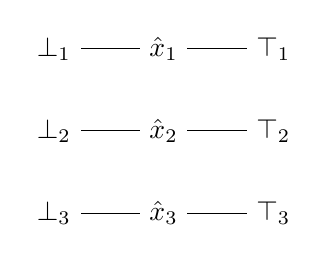
\begin{tikzpicture}[node distance=.75cm]

\node (x1) {$\hat{x}_1$};
\node [below =.5cm of x1] (x2) {$\hat{x}_2$};
\node [below =.5cm of x2] (x3) {$\hat{x}_3$};

\node [right = of x1] (t1) {$\top_1$};
\node [left = of x1] (f1) {$\bot_1$};

\draw [-] (x1) to (t1);
\draw [-] (x1) to (f1);

\node [right = of x2] (t2) {$\top_2$};
\node [left = of x2] (f2) {$\bot_2$};

\draw [-] (x2) to (t2);
\draw [-] (x2) to (f2);

\node [right = of x3] (t3) {$\top_3$};
\node [left = of x3] (f3) {$\bot_3$};

\draw [-] (x3) to (t3);
\draw [-] (x3) to (f3);

\end{tikzpicture}



	}
	
\centering
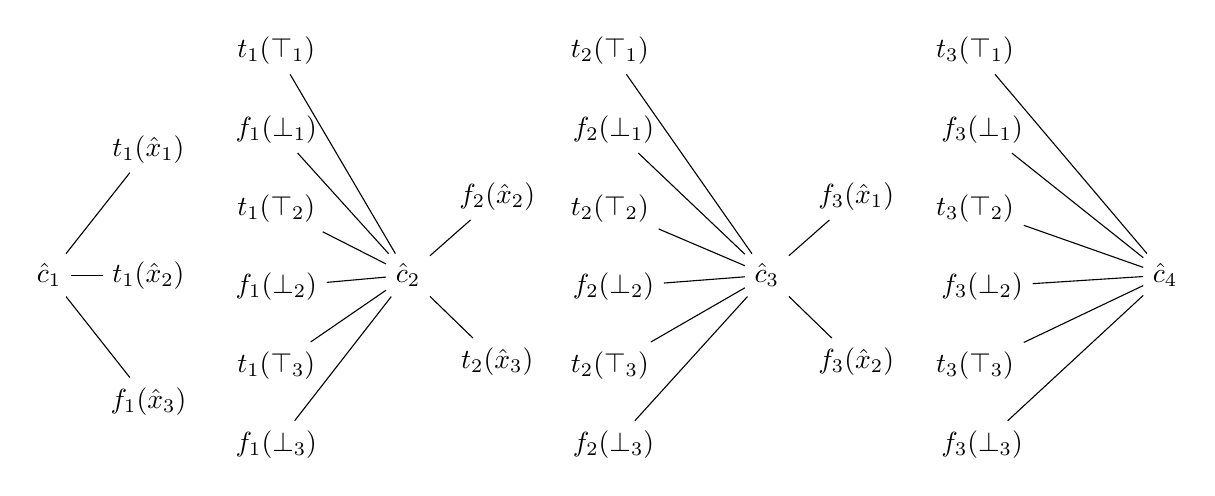
\begin{tikzpicture}[node distance=.3cm]

\node(c1){$\hat{c}_1$};

\node[right =.4cm of c1] (t1x2) {$t_1(\hat{x}_2)$};
\node[above =1cm of t1x2] (t1x1) {$t_1(\hat{x}_1)$};
\node[below =1cm of t1x2] (f1x3) {$f_1(\hat{x}_3)$};

\draw [-] (c1) to (t1x2);
\draw [-] (c1) to (t1x1);
\draw [-] (c1) to (f1x3);


\node[right =.4cm of t1x1, yshift = 0.25cm] (f11) {$f_1(\bot_1)$};
\node[above =.4cm of f11] (t11) {$t_1(\top_1)$};
\node[below =.4cm of f11] (t12) {$t_1(\top_2)$};
\node[below =.4cm of t12] (f12) {$f_1(\bot_2)$};
\node[below =.4cm of f12] (t13) {$t_1(\top_3)$};
\node[below =.4cm of t13] (f13) {$f_1(\bot_3)$};

\node[right = 4cm of c1](c2){$\hat{c}_2$};

\draw [-] (c2) to (t11);
\draw [-] (c2) to (t12);
\draw [-] (c2) to (t13);
\draw [-] (c2) to (f11);
\draw [-] (c2) to (f12);
\draw [-] (c2) to (f13);

\node[right =.25cm of c2, yshift=1cm]  (f2x2) {$f_2(\hat{x}_2)$};
\node[below =1.5cm of f2x2] (t2x3) {$t_2(\hat{x}_3)$};

\draw [-] (c2) to (f2x2);
\draw [-] (c2) to (t2x3);

\node[right =3cm of f11] (f21) {$f_2(\bot_1)$};
\node[right =3cm of t11] (t21) {$t_2(\top_1)$};
\node[right =3cm of t12] (t22) {$t_2(\top_2)$};
\node[right =3cm of f12] (f22) {$f_2(\bot_2)$};
\node[right =3cm of t13] (t23) {$t_2(\top_3)$};
\node[right =3cm of f13] (f23) {$f_2(\bot_3)$};

\node[right = 4cm of c2](c3){$\hat{c}_3$};

\draw [-] (c3) to (t21);
\draw [-] (c3) to (t22);
\draw [-] (c3) to (t23);
\draw [-] (c3) to (f21);
\draw [-] (c3) to (f22);
\draw [-] (c3) to (f23);

\node[right =.25cm of c3, yshift=1cm] (f3x1) {$f_3(\hat{x}_1)$};
\node[below =1.5cm of f3x1] (f3x2) {$f_3(\hat{x}_2)$};

\draw [-] (c3) to (f3x1);
\draw [-] (c3) to (f3x2);

\node[right =3.4cm of f21] (f31) {$f_3(\bot_1)$};
\node[right =3.4cm of t21] (t31) {$t_3(\top_1)$};
\node[right =3.4cm of t22] (t32) {$t_3(\top_2)$};
\node[right =3.4cm of f22] (f32) {$f_3(\bot_2)$};
\node[right =3.4cm of t23] (t33) {$t_3(\top_3)$};
\node[right =3.4cm of f23] (f33) {$f_3(\bot_3)$};

\node[right = 4.5cm of c3](c4){$\hat{c}_4$};

\draw [-] (c4) to (t31);
\draw [-] (c4) to (t32);
\draw [-] (c4) to (t33);
\draw [-] (c4) to (f31);
\draw [-] (c4) to (f32);
\draw [-] (c4) to (f33);

\end{tikzpicture}



\end{block}
}

\only<9>{
\begin{block}{Small subset corresponding to satisfying assignment}

\centering
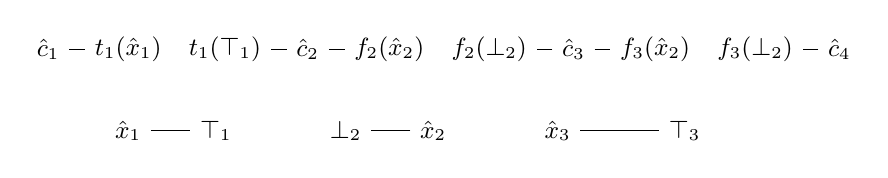
\begin{tikzpicture}
\tikzstyle{every node}=[font=\small]
\node(c1){$\hat{c}_1$};

\node[right =.2cm of c1] (t1x1) {$t_1(\hat{x}_1)$};

\draw [-] (c1) to (t1x1);

\node[right =.1cm of t1x1] (t11) {$t_1(\top_1)$};

%\draw [dashed] (t1x1) to (t11);

\node[right =.2cm of t11](c2){$\hat{c}_2$};

\draw [-] (c2) to (t11);

\node[right =.2cm of c2]  (f2x2) {$f_2(\hat{x}_2)$};

\draw [-] (c2) to (f2x2);

\node[right =.1cm of f2x2] (f22) {$f_2(\bot_2)$};

%\draw [dashed] (f2x2) to (f22);

\node[right = .2cm of f22](c3){$\hat{c}_3$};

\draw [-] (c3) to (f22);

\node[right =.2cm of c3] (f3x2) {$f_3(\hat{x}_2)$};

\draw [-] (c3) to (f3x2);

\node[right =.1cm of f3x2] (f32) {$f_3(\bot_2)$};

%\draw [dashed] (f3x2) to (f32);

\node[right =.2cm of f32](c4){$\hat{c}_4$};

\draw [-] (c4) to (f32);

\node [below =.5cm of t1x1] (x1) {$\hat{x}_1$};

\node [right =.5cm of x1] (t1) {$\top_1$};

\node [right =1cm of t1] (f2) {$\bot_2$};


\node [right =.5cm of f2] (x2) {$\hat{x}_2$};

\node [right =1cm of x2] (x3) {$\hat{x}_3$};


\node [right =1cm of x3] (t3) {$\top_3$};

\draw [-] (x1) to (t1);

\draw [-] (x2) to (f2);


\draw [-] (x3) to (t3);

\end{tikzpicture}


\end{block}
}
\end{frame}

\begin{frame}

\frametitle{Short explanation, long proof}

$$t_a \leftarrow f(f(a,b),f(a,a))$$
$$t_b \leftarrow f(f(b,a),f(b,b))$$


\centering
\begin{tikzpicture}[node distance=2cm]
	\proofnode[align=center]{root} {$a \neq b, t_a = t_b$\\Compatibility proof};
	
	\proofnode[above right of=root,yshift=.25cm]{n5}{$a \neq b, f(a,a) \neq f(b,b), t_a = t_b$};
	\proofnode[above left of=root,yshift=-.25cm]{n7}{$a\neq b, f(a,a) = f(b,b)$};

	\proofnode[above left of=n5,yshift=.25cm]{n3}{$f(a,b) \neq f(b,a), f(a,a) \neq f(b,b), t_a = t_b$};
	\proofnode[above right of=n5,yshift=-.25cm]{n4}{$a \neq b, f(a,b) = f(b,a)$};

	\drawchildren{root}{n5}{n7};
	\drawchildren{n5}{n3}{n4};
	
	\proofnode[right of=root, xshift=2.5cm, align=center]{root2} {$t_a \neq a, a\neq b, b \neq t_b, t_a = t_b$\\Transitivity proof};
\end{tikzpicture}



\end{frame}

\begin{frame}

\frametitle{Congruence Experimental Results}

\begin{itemize}
		\item 3965 proofs of problems of the SMT-LIB benchmark in the QF\_UF logic
\end{itemize}

\begin{table}[h]
\centering
%\setlength{\tabcolsep}{8pt}
\begin{tabular}{l c c c c}
\toprule
\textbf{Method} & \textbf{Compression} & \textbf{Min} & \textbf{Max} & \textbf{Speed}\\ 
\midrule

EqGraph & \textbf{5.350} \% & -18.302 \% & \textbf{81.347} \% & 0.343 \\ 
Proof Forest &  5.196 \% & -43.985 \% & 77.202 \% & 0.611 \\ 
DAGify & 3.368 \% & \textbf{0.0} \% & 14.433 \% & \textbf{1.655} \\ 

\bottomrule
%\hline
\end{tabular}
\caption{Compression Results}
\label{tab:congruence_results}
\end{table}

\begin{table}[h]
\centering
%\setlength{\tabcolsep}{8pt}
\begin{tabular}{l c c}
\toprule
\textbf{Congruence Graph} & \textbf{Compressed} & \textbf{Compression} \\ 
\midrule

Equation Graph & 12.42 \% & 28.34 \% \\ 
Proof Forest & 11.459 \% & 28.69 \% \\ 

\bottomrule
%\hline
\end{tabular}
\caption{Explanation Size Results}
\label{tab:explanation_results}
\end{table}

\end{frame}

\begin{frame}
\begin{figure}[h]
	\centering
	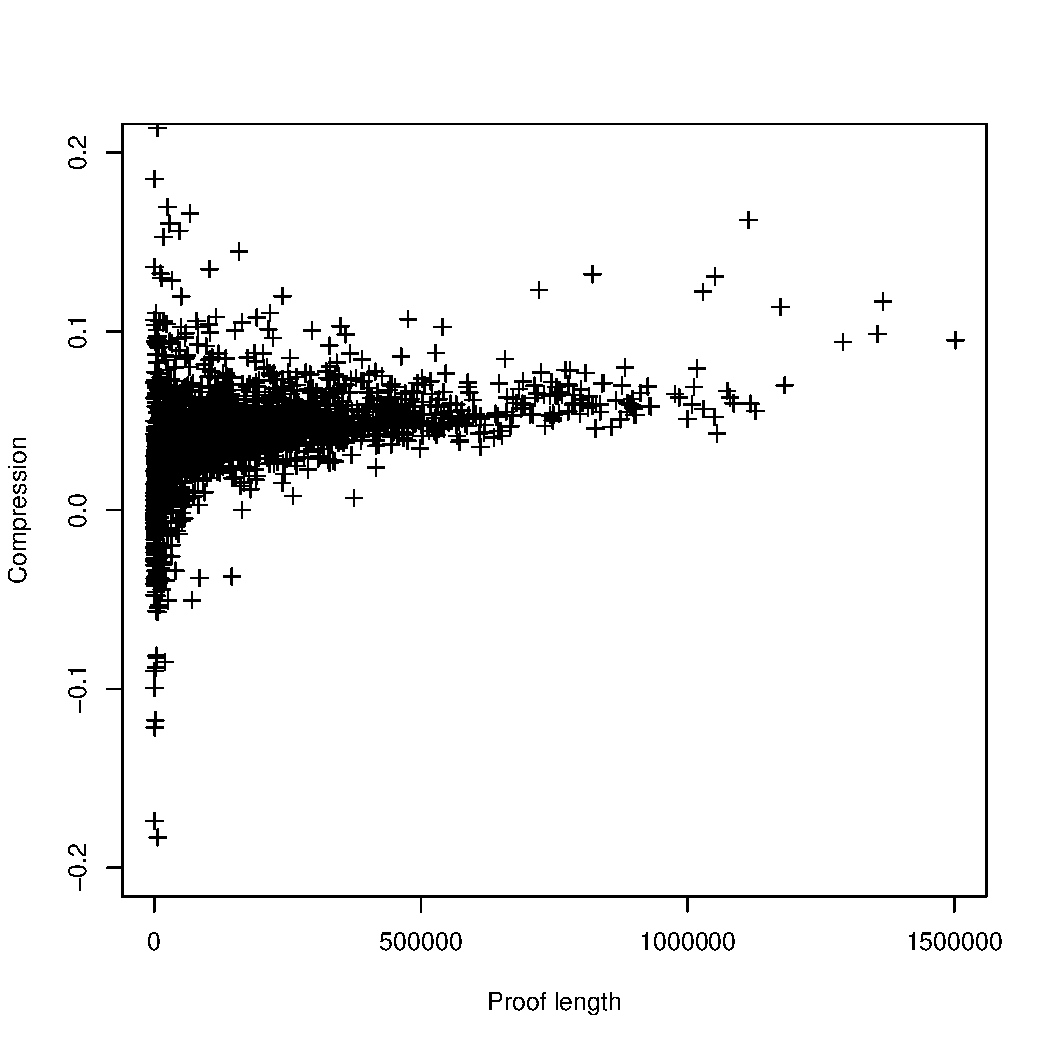
\includegraphics[scale=0.5]{../latex/chapters/congruence/figures/compression_vs_length.pdf}
	\caption{Compression vs Proof Length}
	\label{fig:congruence_compression}
\end{figure}

\end{frame}

\begin{frame}

\frametitle{Space Compression Results}

\begin{itemize}
	\item VeriT: Problems from SMT-lib
	\item TraceCheck: Problems from SATLIB, computed with PicoSAT
\end{itemize}

\begin{table}[tb]
	\centering
	\setlength{\tabcolsep}{8pt}
	\begin{tabular}{lrrr}
		\toprule
		%\textbf{Name} & \textbf{Number of proofs} & \textbf{Maximum length} & \textbf{Average length} \\ 
		\textbf{Name} & \textbf{Number of} & \textbf{Maximum} & \textbf{Average} \\ 
		              & \textbf{proofs}    & \textbf{length}  & \textbf{length} \\
		\midrule
		TraceCheck$_1$ & 2239 & 90756   & 5423   \\
		TraceCheck$_2$ & 215	& 1768249 & 268863 \\
    veriT$_1$ & 4187 & 2241042 & 103162 \\
    veriT$_2$ & 914  & 120075  & 5391  \\ 
		\bottomrule   
	\end{tabular}
	\caption{Proof Benchmark Sets}
	\label{tab:benchmarks}
\end{table}


\end{frame}

\begin{frame}

\frametitle{Space Compression Results}

\begin{table}[tb]
\centering
%\setlength{\tabcolsep}{8pt}
\begin{tabular}{l c c}
\toprule
\textbf{Algorithm} & \textbf{Relative} & \textbf{Speed}\\ 
Heuristic & \textbf{Performance} (\%) & (nodes/ms)\\ 
\midrule

\textbf{Bottom-Up} & & \\
Children & 17.52 & \textbf{88.6} \\ 
LastChild & \textbf{26.31} & 84.5 \\ 
Distance(1) & 9.46 & 21.2 \\ 
Distance(3) & -0.40 & 0.5\\ 

\midrule

\textbf{Top-Down} & & \\
Children & -27.47 & 0.3 \\
LastChild & -31.98 & 1.9 \\
Distance(1) & -70.14 & 0.6 \\ 
Distance(3) & \textbf{-74.33} & \textbf{0.1}\\ 

\bottomrule
%\hline
\end{tabular}
\caption{Experimental Results}
\label{tab:results}
\end{table}

\end{frame}

\begin{frame}
	\frametitle{Construct Order Top-Down}
	\centering
	Maximum number of nodes in memory:
		\alt<1>{0}{\alt<2>{1}{\alt<3>{2}{\alt<4-7>{3}{\alt<8-11>{4}{\alt<12-15>{5}{6}}}}}} \\[1cm]
	\begin{tikzpicture}[node distance=1cm]
		\proofnodeBWHidden{root};
		
		\proofnodeBWHidden[above left=of root,xshift=-1.5cm]{n4};
		\proofnodeBWHidden[above right=of root,xshift=1.5cm]{n15};
		\proofnodeBWHidden[above =of root,yshift=0.5cm]{n11};

		\proofnodeBWHidden[above left=of n4]{h1};
		\proofnodeBWHidden[above right=of n15]{h2};
		\proofnodeBWHidden[above left=of n11]{h3};
		\proofnodeBWHidden[above right=of n11]{h4};
		
		\proofnodeBW[above left=of h1]{n3};
		\proofnodeBW[above right=of h2]{n14};
		\proofnodeBW[right=of n3,xshift=1.6cm]{n7};
		\proofnodeBW[left=of n14,xshift=-1.6cm]{n10};

		\withchildrenBW{n3} {n1} {n2};
		\withchildrenBW{n7} {n5} {n6};
		\withchildrenBW{n10} {n8} {n9};
		\withchildrenBW{n14} {n12} {n13};
		
		\blacknode<2-4>{n1};
		\blacknode<3,4>{n2};
		\blacknode<4-20>{n3};
		\whitenode<3-20>{n4};
		\draw<3->[proof edge] (n4) -- (n3);
		
		\blacknode<6-8>{n12};
		\blacknode<7,8>{n13};
		\blacknode<8-22>{n14};
		\whitenode<7->{n15};
		\draw<7->[proof edge] (n15) -- (n14);
		
		\blacknode<10-12>{n5};
		\blacknode<11,12>{n6};
		\blacknode<12-18>{n7};
		\whitenode<11->{n11};
		\draw<11->[proof edge] (n11) -- (n7);
		
		\blacknode<14-16>{n8};
		\blacknode<15,16>{n9};
		\blacknode<16-18>{n10};
		\draw<15->[proof edge] (n11) -- (n10);
		
		\draw<16->[proof edge] (n4) -- (n11);
		\draw<16->[proof edge] (n15) -- (n11);
		
		\blacknode<18-22>{n11};
		\draw<18->[proof edge] (root) -- (n4);
		\draw<18->[proof edge] (root) -- (n15);
		\whitenode<18->{root}
		
		\blacknode<20->{n4};
		
		\blacknode<22->{n15};
		
		\blacknode<24>{root};
	\end{tikzpicture}
\end{frame}

\begin{frame}
	\frametitle{Construct Order Bottom-Up}
	\centering
	Maximum number of nodes in memory:
		\alt<1-4>{0}{\alt<5>{1}{\alt<6>{2}{\alt<7-12>{3}{\alt<13-17>{4}{5}}}}} \\[1cm]
	\begin{tikzpicture}[node distance=1cm]
		\rootnodeBW;

		\proofnodeBW[above left=of root,xshift=-1.5cm]{n4};
		\proofnodeBW[above right=of root,xshift=1.5cm]{n15};
		\draw[proof edge] (root) -- (n4);
		\draw[proof edge] (root) -- (n15);
				
		\proofnodeBWHidden[above =of root,yshift=0.5cm]{n11};

		\proofnodeBWHidden[above left=of n4]{h1};
		\proofnodeBWHidden[above right=of n15]{h2};
		\proofnodeBWHidden[above left=of n11]{h3};
		\proofnodeBWHidden[above right=of n11]{h4};
		
		\proofnodeBWHidden[above left=of h1]{n3};
		\proofnodeBWHidden[above right=of h2]{n14};
		\proofnodeBWHidden[right=of n3,xshift=1.6cm]{n7};
		\proofnodeBWHidden[left=of n14,xshift=-1.6cm]{n10};

		\proofnodeBWHidden[above left of=n3]{n1};
		\proofnodeBWHidden[above right of=n3]{n2};
		\proofnodeBWHidden[above left of=n7]{n5};
		\proofnodeBWHidden[above right of=n7]{n6};
		
		\proofnodeBWHidden[above left of=n10]{n8};
		\proofnodeBWHidden[above right of=n10]{n9};
		
		\proofnodeBWHidden[above left of=n14]{n12};
		\proofnodeBWHidden[above right of=n14]{n13};
			
		\waitingnode<2-32>{root};
		\whitenode<2->{n11};
		\whitenode<2->{n3};
		\whitenode<2->{n14};
		\draw<2->[proof edge] (n4) -- (n3);
		\draw<2->[proof edge] (n4) -- (n11);
		\draw<2->[proof edge] (n15) -- (n11);
		\draw<2->[proof edge] (n15) -- (n14);
		
		\waitingnode<3->{n15};
		\whitenode<3->{n10};
		\whitenode<3->{n7};
		\whitenode<3->{n12};
		\whitenode<3->{n13};
		\draw<3->[proof edge] (n14) -- (n12);
		\draw<3->[proof edge] (n14) -- (n13);
		\draw<3->[proof edge] (n11) -- (n7);
		\draw<3->[proof edge] (n11) -- (n10);
		
		
		\waitingnode<4-7>{n14};
		
		\blacknode<5-7>{n12};
		\blacknode<6,7>{n13};
		\blacknode<7-22>{n14};
		
		\waitingnode<9-20>{n11};
		\whitenode<9->{n5};
		\whitenode<9->{n6};
		\whitenode<9->{n8};
		\whitenode<9->{n9};
		\draw<9->[proof edge] (n7) -- (n5);
		\draw<9->[proof edge] (n7) -- (n6);
		\draw<9->[proof edge] (n10) -- (n8);
		\draw<9->[proof edge] (n10) -- (n9);
		
		\waitingnode<10-13>{n7};
		\blacknode<11-13>{n6};
		\blacknode<12,13>{n5};
		\blacknode<13-20>{n7};
		
		\waitingnode<15-18>{n10};
		\blacknode<16-18>{n8};
		\blacknode<17,18>{n9};
		\blacknode<18-20>{n10};
		
		\blacknode<20-30>{n11};
		\blacknode<22->{n15};
		
		\waitingnode<24-31>{n4};
		\whitenode<24->{n1};
		\whitenode<24->{n2};
		\draw<24->[proof edge] (n3) -- (n1);
		\draw<24->[proof edge] (n3) -- (n2);
		
		\waitingnode<25-28>{n3};
		\blacknode<26-28>{n1};
		\blacknode<27,28>{n2};
		\blacknode<28-30>{n3};
		
		\blacknode<30->{n4};
		
		\blacknode<32>{root};
		
	\end{tikzpicture}

\end{frame}

\end{document}
